\documentclass[journal,twocolumn]{IEEEtran}

% ── Core packages ─────────────────────────────────────────────────────
\usepackage[T1]{fontenc}
\usepackage{amsmath,amssymb,amsfonts}
\usepackage{algorithmic}
\usepackage{algorithm}
\usepackage{graphicx}
\usepackage{textcomp}
\usepackage{xcolor}
\usepackage{booktabs}
\usepackage{cite}
\usepackage{multirow}
\usepackage{array}
\usepackage{bm}
\usepackage{balance}
\usepackage[caption=false,font=footnotesize]{subfig}
\usepackage{url}

\graphicspath{{./}{./outputs_joint_ao/ieee_plots/}}

% ── Math shortcuts ────────────────────────────────────────────────────
\newcommand{\vect}[1]{\mathbf{#1}}
\newcommand{\mat}[1]{\mathbf{#1}}
\newcommand{\E}{\mathbb{E}}
\newcommand{\R}{\mathbb{R}}
\newcommand{\C}{\mathbb{C}}
\DeclareMathOperator{\diag}{diag}
\DeclareMathOperator{\Tr}{Tr}
\DeclareMathOperator*{\argmax}{arg\,max}
\DeclareMathOperator*{\argmin}{arg\,min}
\newcommand{\dBm}{\,\text{dBm}}
\newcommand{\dB}{\,\text{dB}}
\newcommand{\GHz}{\,\text{GHz}}

\begin{document}

% ══════════════════════════════════════════════════════════════════════
% TITLE
% ══════════════════════════════════════════════════════════════════════

\title{Intelligent Reflecting Surface Assisted Anti-Jamming Communications in THz Wideband Systems: A Fuzzy WoLF-PHC Learning Approach with Hybrid Beamforming}

\author{Anuprabh Singh%
\thanks{Anuprabh Singh is with the Department of Electronics and Communication Engineering, National Institute of Technology, Warangal 506004, India (e-mail: anuprabh@student.nitw.ac.in).}}

\maketitle

% ══════════════════════════════════════════════════════════════════════
% ABSTRACT
% ══════════════════════════════════════════════════════════════════════

\begin{abstract}
Wideband terahertz (THz) communications offer multi-gigahertz spectrum access but are acutely vulnerable to targeted jamming owing to their narrow, highly directional beams. This paper proposes a unified framework for intelligent reflecting surface (IRS)-assisted anti-jamming in THz wideband systems, jointly optimizing transmit power allocation, IRS phase shifts, and hybrid analog-digital beamforming against a smart adaptive jammer. The resulting optimization problem is non-convex, high-dimensional, and subject to a dynamic adversary with unknown strategy; we decompose it via a three-block alternating optimization (AO) framework that solves each block in closed form or via reinforcement learning (RL). The novel fuzzy Win-or-Learn-Fast policy hill-climbing (WoLF-PHC) RL agent manages discrete power allocation using a 27-component fuzzy state abstraction and win/loss-adaptive learning rates, converging to a mixed strategy that is inherently unpredictable to a jammer monitoring action history. The THz system model incorporates $f_c=100\,\text{GHz}$, $B=10\,\text{GHz}$ wideband OFDM (64 subcarriers), a 64-antenna sub-connected base station with $N_\mathrm{RF}=8$ RF chains, and a 256-element sub-array phase-dependent partial-connection (SPDP) RIS for wideband beam-squint compensation. Evaluated over five independent seeds with 600 training episodes each, the proposed method achieves $11.87\,\text{bits/s/Hz}$ system rate and $81.6\%$ SINR protection, outperforming classical Q-learning ($8.25\,\text{bits/s/Hz}$, $49.0\%$), DQN ($8.23\,\text{bits/s/Hz}$, $49.1\%$), and the deterministic AO baseline ($7.89\,\text{bits/s/Hz}$, $43.2\%$) with substantially lower seed variance. Comprehensive parameter sweeps over transmit power, RIS size, SINR threshold, and jammer power confirm consistent gains and a pronounced regime transition: deterministic optimization leads at low jammer power, whereas WoLF-PHC dominates under stronger adversarial pressure.
\end{abstract}

\begin{IEEEkeywords}
Anti-jamming, intelligent reflecting surface, terahertz communications, hybrid beamforming, reinforcement learning, WoLF-PHC, beam squint.
\end{IEEEkeywords}

% ══════════════════════════════════════════════════════════════════════
\section{Introduction}
\label{sec:intro}
% ══════════════════════════════════════════════════════════════════════

\IEEEPARstart{T}{Hz} systems provide massive bandwidth but are highly vulnerable to adaptive jamming because links are narrow-beam, frequency selective, and sensitive to beam squint. IRS-assisted anti-jamming is promising~\cite{wu2019intelligent,wu2021irs_survey,renzo2020smart}, but prior RL-based studies are largely narrowband and do not jointly address wideband THz beam squint, sub-connected hybrid beamforming constraints, and smart jammers that exploit predictable control policies~\cite{yang2021irs,su2023wideband,yan2023beamforming}. This work closes that gap with a unified THz-OFDM formulation and a robust mixed-strategy controller.

\subsection{Contributions}

The main contributions are:

\begin{enumerate}
\item \textbf{Joint THz anti-jamming formulation:} We jointly optimize power allocation, SPDP-RIS phase control, and sub-connected hybrid beamforming for a $100$~GHz, $10$~GHz-bandwidth THz-OFDM system with adaptive jamming.
\item \textbf{Three-block RL+AO solver:} We combine RL for discrete power control (42 actions) with closed-form AO updates for IRS phases and SVD/MVDR updates for hybrid beamforming.
\item \textbf{Fuzzy WoLF-PHC with real-data validation:} A 27-component fuzzy state abstraction and win/loss-adaptive policy updates improve robustness against policy-exploiting jammers; five-seed, 600-episode experiments and real sweeps show $44\%$ rate and $66\%$ protection gains over the best baseline.
\end{enumerate}

\emph{Notation:} Bold lower/uppercase denotes vectors/matrices; $(\cdot)^H$, $|\cdot|$, $\|\cdot\|$, $\diag(\cdot)$, and $\mathbf{1}\{\cdot\}$ have standard meanings.

% ══════════════════════════════════════════════════════════════════════
\section{System Model and Problem Formulation}
\label{sec:system}
% ══════════════════════════════════════════════════════════════════════

\subsection{System Description}

We consider a downlink THz-OFDM system comprising a $N=64$-antenna base station (BS) with $N_{\text{RF}}=8$ RF chains, a 256-element ($16\!\times\!16$) SPDP-RIS, $K=4$ single-antenna users, and a colluding 2-antenna smart jammer, operating at $f_c=100\,\text{GHz}$ with bandwidth $B=10\,\text{GHz}$ and $M_{\text{sc}}=64$ OFDM subcarriers. The BS employs a sub-connected hybrid analog-digital architecture in which each RF chain drives $N_{\text{per}}=N/N_{\text{RF}}=8$ dedicated antennas, balancing hardware complexity with spatial degrees of freedom. The IRS is deployed to establish a reflected path between the BS and users, augmenting the direct link and enabling passive spatial filtering of the jamming signal.

\subsection{Signal Model}

Let $\mat{G}[m] \in \C^{M \times N}$ denote the BS-IRS channel at subcarrier $m$, $\vect{g}_{ru,k}[m] \in \C^{M}$ the IRS-to-user-$k$ channel, $\vect{g}_{bu,k}[m] \in \C^{N}$ the direct BS-to-user-$k$ channel, and $\vect{h}_{J,k} \in \C^{N_J}$ the jammer-to-user-$k$ channel. The IRS introduces a diagonal reflection matrix $\bm{\Phi}[m] = \diag(e^{j\theta_1[m]}, \ldots, e^{j\theta_M[m]})$ at subcarrier $m$, where the SPDP architecture allows subcarrier-level phase control to compensate beam squint (Section~\ref{sec:thz}).

The received signal at user $k$ on subcarrier $m$ is
\begin{align}
y_k[m] &= \underbrace{\left(\vect{g}_{ru,k}^H[m]\bm{\Phi}[m]\mat{G}[m] + \vect{g}_{bu,k}^H[m]\right)\vect{w}_k[m]\sqrt{P_k}\,s_k}_{\text{desired signal}} \nonumber\\
&+ \underbrace{\sum_{i \neq k}\left(\vect{g}_{ru,k}^H[m]\bm{\Phi}[m]\mat{G}[m] + \vect{g}_{bu,k}^H[m]\right)\vect{w}_i[m]\sqrt{P_i}\,s_i}_{\text{inter-user interference}} \nonumber\\
&+ \underbrace{\sqrt{P_{J,k}}\,\vect{h}_{J,k}^H\vect{z}_k\,j_k}_{\text{jamming}} + n_k \label{eq:signal}
\end{align}
where $\vect{w}_k[m] \in \C^{N}$ is the beamforming vector, $P_k$ is the allocated power, $s_k$ is the unit-power data symbol, $P_{J,k}$ is the instantaneous jamming power toward user $k$, $\vect{z}_k$ is the jammer's spatial precoder, $j_k$ is the jamming symbol, and $n_k \sim \mathcal{CN}(0, \sigma^2)$ is additive white Gaussian noise with variance $\sigma^2 = k_B T B / M_{\text{sc}} + F_{\text{NF}}$, where $k_B$ is Boltzmann's constant, $T = 290$~K, and $F_{\text{NF}} = 10\,\text{dB}$ is the receiver noise figure.

\subsection{SINR and System Rate}

The effective channel for user $k$ at subcarrier $m$ is
\begin{equation}
\vect{h}_{\text{eff},k}[m] = \mat{G}^H[m]\bm{\Phi}^H[m]\vect{g}_{ru,k}[m] + \vect{g}_{bu,k}[m].
\label{eq:heff}
\end{equation}

The received SINR at user $k$ on subcarrier $m$ is
\begin{equation}
\text{SINR}_k[m] = \frac{P_k |\vect{h}_{\text{eff},k}^H[m]\vect{w}_k[m]|^2}{\displaystyle\sum_{i \neq k}P_i|\vect{h}_{\text{eff},k}^H[m]\vect{w}_i[m]|^2 + P_{J,k}|\vect{h}_{J,k}^H\vect{z}_k|^2 + \sigma^2}.
\label{eq:sinr}
\end{equation}

The per-user rate averaged over subcarriers is
\begin{equation}
R_k = \frac{1}{M_{\text{sc}}}\sum_{m=1}^{M_{\text{sc}}} \log_2(1 + \text{SINR}_k[m])
\label{eq:rate}
\end{equation}
and the system sum-rate is $R_{\text{sum}} = \sum_{k=1}^{K} R_k$.

The SINR protection level measures quality-of-service (QoS) satisfaction:
\begin{equation}
\eta_{\text{prot}} = \frac{1}{K \cdot M_{\text{sc}}}\sum_{k=1}^{K}\sum_{m=1}^{M_{\text{sc}}} \mathbf{1}\{\text{SINR}_k[m] \geq \gamma_{\min}\}
\label{eq:protection}
\end{equation}
where $\gamma_{\min}$ is the minimum SINR threshold.

\subsection{Problem Formulation}

Substituting the hybrid beamformer decomposition $\vect{w}_k[m] = \mat{F}_{\text{RF}}\vect{f}_{BB,k}[m]$ into the SINR expression~\eqref{eq:sinr}, the joint optimization over power allocation, IRS phase shifts, and hybrid beamforming is formulated as
\begin{subequations}
\begin{align}
\max_{\{P_k\}, \{\bm{\Phi}[m]\}, \mat{F}_{\text{RF}}, \{\vect{f}_{BB,k}[m]\}} \quad & R_{\text{sum}} \label{eq:obj}\\
\text{s.t.} \quad & \sum_{k=1}^{K} P_k \leq P_{\max} \label{eq:power}\\
& \text{SINR}_k[m] \geq \gamma_{\min},\ \forall k, m \label{eq:qos}\\
& |\Phi_{m,m}[n]| = 1,\ \forall m, n \label{eq:unit}\\
& [\mat{F}_{\text{RF}}]_{ij} = 0,\ \forall (i,j) \notin \mathcal{S}_{\text{BC}} \label{eq:bc}\\
& |[\mat{F}_{\text{RF}}]_{ij}| = \tfrac{1}{\sqrt{N_{\text{per}}}},\ \forall (i,j) \in \mathcal{S}_{\text{BC}} \label{eq:cm}\\
& \|\mat{F}_{\text{RF}}\vect{f}_{BB,k}[m]\|^2 \leq 1,\ \forall k, m \label{eq:pn}
\end{align}
\end{subequations}
where~\eqref{eq:power} is the total power budget, \eqref{eq:qos} is the per-user QoS constraint, \eqref{eq:unit} is the unit-modulus constraint on IRS elements, \eqref{eq:bc} enforces the block-diagonal (sub-connected) structure of the analog precoder with $\mathcal{S}_{\text{BC}}$ denoting the support set of non-zero entries, \eqref{eq:cm} is the constant-modulus constraint on the $N_{\text{per}} = N/N_{\text{RF}}$ non-zero entries per column, and~\eqref{eq:pn} ensures unit-norm beamforming vectors so that $P_k$ is the sole power scaling.

Problem~\eqref{eq:obj}--\eqref{eq:pn} is non-convex and NP-hard due to the coupled optimization variables, the unit-modulus IRS constraint~\eqref{eq:unit}, and the constant-modulus analog precoder constraint~\eqref{eq:cm}. Critically, the jammer's transmit power, spatial precoder, and targeting strategy are dynamic and unknown, making model-based optimization or convex relaxations ineffective in practice. We therefore adopt a hybrid RL+AO formulation: RL handles the combinatorial, model-free power allocation under adversarial uncertainty, while closed-form AO updates efficiently handle the continuous-valued IRS phase and beamforming blocks at each RL step.

% ══════════════════════════════════════════════════════════════════════
\section{THz Channel Model and Wideband Beamforming}
\label{sec:thz}
% ══════════════════════════════════════════════════════════════════════

\subsection{THz Channel Model}

THz channels are characterized by frequency-selective behavior arising from molecular absorption, which creates spectral windows of low attenuation separated by opacity bands. The BS-IRS channel at subcarrier $m$ follows a geometry-based Saleh-Valenzuela model~\cite{su2023wideband}:
\begin{equation}
\mat{G}[m] = \sqrt{\frac{N M}{L_{\text{path}}}} \sum_{\ell=1}^{L_{\text{path}}} \alpha_\ell(f_m)\, \vect{a}_{\text{RIS}}(\phi_\ell, f_m) \vect{a}_{\text{BS}}^H(\psi_\ell, f_m)
\label{eq:thz_channel}
\end{equation}
where $L_{\text{path}}$ is the number of propagation paths, $\alpha_\ell(f_m)$ is the complex path gain at subcarrier frequency $f_m = f_c + (m - M_{\text{sc}}/2)\Delta f$ with subcarrier spacing $\Delta f = B/M_{\text{sc}}$, and $\vect{a}_{\text{RIS}}$, $\vect{a}_{\text{BS}}$ are frequency-dependent array steering vectors. The frequency dependence of the steering vectors is the root cause of beam squint, as the spatial angle-of-arrival/departure at which constructive interference occurs shifts with frequency.

\subsection{Path Loss and Molecular Absorption}

The THz path loss at frequency $f$ and distance $d$ is
\begin{equation}
\text{PL}(f, d) = \left(\frac{4\pi f d}{c}\right)^2 e^{\kappa_{\text{abs}}(f) d}
\label{eq:pathloss}
\end{equation}
where $c$ is the speed of light and $\kappa_{\text{abs}}(f)$ is the molecular absorption coefficient. Unlike microwave channels, $\kappa_{\text{abs}}(f)$ varies significantly within the 10\,GHz bandwidth, introducing per-subcarrier attenuation diversity that the OFDM system must accommodate.

\subsection{SPDP-RIS Architecture for Beam-Squint Compensation}

To mitigate wideband beam squint, we adopt the sub-array phase-dependent partial-connection (SPDP) architecture~\cite{su2023wideband}. The $M$ RIS elements are partitioned into $Q = Q_1 \times Q_2 = 64$ sub-arrays (each of $M_s = M/Q = 4$ elements), each with a true-time-delay (TTD) unit and per-element phase shifters:
\begin{equation}
\theta_{q,i}[m] = \theta_{q,i}^{\text{base}} + 2\pi f_m \tau_q
\label{eq:spdp}
\end{equation}
where $\theta_{q,i}^{\text{base}}$ is the base phase and $\tau_q$ is the TTD delay for sub-array $q$. This keeps beam direction consistent across subcarriers and avoids edge-subcarrier gain loss.

\subsection{Hybrid Beamforming at the BS}

The BS employs a sub-connected hybrid architecture with $N_{\text{RF}} = 8$ RF chains, each connected exclusively to $N_{\text{per}} = N/N_{\text{RF}} = 8$ antennas. This eliminates the inter-chain interference of fully-connected architectures at the cost of reduced degrees of freedom, a trade-off well-suited to the sparse THz channel. The beamforming vector decomposes as
\begin{equation}
\vect{w}_k[m] = \mat{F}_{\text{RF}} \vect{f}_{BB,k}[m]
\label{eq:hybrid_bf}
\end{equation}
where $\mat{F}_{\text{RF}} \in \C^{N \times N_{\text{RF}}}$ is the frequency-flat analog precoder (block-diagonal, constant-modulus entries) and $\vect{f}_{BB,k}[m] \in \C^{N_{\text{RF}}}$ is the per-subcarrier digital precoder. The digital precoder adopts a max-SINR (MVDR) design. For user $k$ at subcarrier $m$, the interference-plus-noise covariance is
\begin{equation}
\mat{R}_k[m] = \sigma^2\mat{I} + \sum_{i \neq k}P_i\,\tilde{\vect{h}}_i[m]\tilde{\vect{h}}_i^H[m]
\label{eq:Rk}
\end{equation}
where $\tilde{\vect{h}}_k[m] = \mat{F}_{\text{RF}}^H\vect{h}_{\text{eff},k}[m]$ is the compressed effective channel. The MVDR precoder is
\begin{equation}
\vect{f}_{BB,k}[m] = \frac{\mat{R}_k^{-1}[m]\tilde{\vect{h}}_k[m]}{\|\mat{R}_k^{-1}[m]\tilde{\vect{h}}_k[m]\|}.
\label{eq:mvdr}
\end{equation}

% ══════════════════════════════════════════════════════════════════════
\section{Reinforcement Learning Framework}
\label{sec:rl}
% ══════════════════════════════════════════════════════════════════════

\subsection{Three-Block AO Decomposition}

The joint optimization~\eqref{eq:obj}--\eqref{eq:pn} couples three structurally distinct variable blocks: the discrete power allocation $\{P_k\}$, the continuous unit-modulus IRS phases $\{\bm{\Phi}[m]\}$, and the hybrid beamformer $\{\mat{F}_{\text{RF}}, \vect{f}_{BB,k}[m]\}$. Rather than relaxing any block, we decompose the problem into three alternating subproblems that are each tractable when the other two are fixed:

\begin{enumerate}
\item \textbf{Block 1 — Power allocation (RL):} The RL agent selects a power allocation action from $\mathcal{A}$ ($|\mathcal{A}|=42$ actions) mapping to discrete power fractions and distribution modes. This block handles the combinatorial structure and model-free nature of the adversarial environment.
\item \textbf{Block 2 — IRS phase shifts (closed-form AO):} Given $\{P_k\}$ and $\mat{F}_{\text{RF}}$, the IRS phases that maximize aggregate desired signal power are computed in closed form per element, eliminating the need for iterative solvers.
\item \textbf{Block 3 — Hybrid beamforming (SVD + MVDR):} Given $\{P_k\}$ and $\{\bm{\Phi}[m]\}$, the analog precoder is updated by SVD-based dominant-subspace projection under the constant-modulus constraint, and the digital precoder is re-solved via MVDR~\eqref{eq:mvdr}.
\end{enumerate}

Blocks 2 and 3 alternate for $N_{\text{AO}}=3$ inner iterations per RL step, ensuring the continuous variables track the RL agent's power decision at negligible computational overhead. Block~1 is updated at the episode boundary through environment interaction.

\subsubsection{Block 2: IRS Phase Optimization via AO}
Given $\{P_k\}$ and $\mat{F}_{\text{RF}}$, the IRS phases are updated in closed form by maximizing the sum of desired signal magnitudes. For each element $i$:
\begin{equation}
c_i = \sum_{k=1}^{K}\sqrt{P_k}\,g_{ru,k}^*[i]\cdot(\mat{G}\vect{w}_k)[i], \quad \theta_i = -\angle(c_i)
\label{eq:ao_phase}
\end{equation}
where $\vect{w}_k = \mat{F}_{\text{RF}}\vect{f}_{BB,k}$ uses the current analog precoder. The optimal SPDP direction is also selected from $K+1$ candidate user directions to maximize system rate, ensuring wideband beam-squint compensation.

\subsubsection{Block 3: Analog Precoder Update via SVD}
Since $\mat{F}_{\text{RF}}$ is frequency-flat, we aggregate the effective channel over reference subcarriers $\mathcal{M}_{\text{ref}}$ as $\overline{\mat{H}} = \sum_{m \in \mathcal{M}_{\text{ref}}} \vect{H}_{\text{eff}}^H[m]$. For sub-array $p$, the row partition $\overline{\mat{H}}_p$ is SVD-decomposed and the analog column is updated as $[\mat{F}_{\text{RF}}]_p = \exp(j\angle\vect{u}_p)/\sqrt{N_{\text{per}}}$ (unit-modulus projection), then $\{\vect{f}_{BB,k}[m]\}$ is re-solved via MVDR~\eqref{eq:mvdr}.

\subsection{State Representation}

We compress the observation into a 3-feature state $\vect{f} = [f_{\text{pj}}, f_{\text{ch}}, f_{\text{sinr}}] \in [0,1]^3$:

\textbf{Jammer pressure:}
\begin{equation}
f_{\text{pj}} = \text{norm}_{[15,40]}\!\left(0.6\overline{P_J}\,[\dBm] + 0.4\max_k P_{J,k}\,[\dBm]\right)
\end{equation}

\textbf{Channel quality:}
\begin{equation}
f_{\text{ch}} = \text{norm}_{[-100,-40]}\!\left(0.75\overline{\|\vect{h}_k\|^2}\,[\dB] + 0.25(1 - \text{spread})\right)
\end{equation}

\textbf{SINR health:}
\begin{equation}
f_{\text{sinr}} = \text{norm}_{[-10,30]}\!\left(0.5\overline{\text{SINR}_k}\,[\dB] + 0.5\min_k\text{SINR}_k\,[\dB]\right)
\end{equation}

Each feature is quantized into $B_q=8$ bins for tabular baselines ($512$ states). WoLF-PHC instead uses fuzzy memberships for smooth interpolation.

\subsection{Fuzzy State Aggregation}

Each feature $x \in [0,1]$ is mapped to three triangular memberships with centers $\{0,0.5,1.0\}$:
\begin{equation}
\mu_i(x) = \frac{\max(0, 1 - |x - c_i|/\Delta)}{\sum_j \max(0, 1 - |x - c_j|/\Delta)}
\label{eq:fuzzy}
\end{equation}
where $\Delta = 0.5$ is the spread parameter. The joint fuzzy membership vector has $3^3 = 27$ components:
\begin{equation}
\psi_\ell(\vect{f}) = \mu_i(f_{\text{pj}}) \cdot \mu_j(f_{\text{ch}}) \cdot \mu_k(f_{\text{sinr}}), \quad \ell = 9i + 3j + k.
\label{eq:fuzzy_joint}
\end{equation}

This smooths state transitions and improves robustness.

\subsection{Proposed Fuzzy WoLF-PHC Algorithm}

WoLF-PHC~\cite{bowling2002wolf} learns faster when losing and slower when winning. The fuzzy version maintains $Q_\ell(s,a)$, policy $\pi_\ell(a)$, and average policy $\bar{\pi}_\ell(a)$ for 27 fuzzy states.

\subsubsection{Fused Q-Value}
The effective Q-value at state $s$ is computed as a fuzzy-weighted combination:
\begin{equation}
\text{FQ}(s, a) = \sum_{\ell=1}^{27}\psi_\ell(s) \cdot Q_\ell(s, a).
\label{eq:fused_q}
\end{equation}

\subsubsection{Q-Update}
For each active fuzzy state $\ell$ (where $\psi_\ell > 0$):
\begin{equation}
Q_\ell(s,a) \leftarrow Q_\ell(s,a) + \alpha\psi_\ell\left[r + \gamma\max_{a'}\text{FQ}(s',a') - Q_\ell(s,a)\right]
\label{eq:q_update}
\end{equation}
where $\alpha = 0.01$ is the learning rate and $\gamma = 0.9$ is the discount factor.

\subsubsection{WoLF-PHC Policy Update}
The win-or-learn-fast mechanism adapts the learning speed based on performance:
\begin{equation}
\xi = \begin{cases}
\xi_{\text{win}} = 0.01 & \text{if } \E_\pi[Q] > \E_{\bar{\pi}}[Q] \\
\xi_{\text{loss}} = 0.04 & \text{otherwise}
\end{cases}
\label{eq:wolf}
\end{equation}

The policy is updated with step size $\delta = \xi \cdot \psi_\ell / L$:
\begin{align}
\pi_\ell(a^*) &\leftarrow \pi_\ell(a^*) + \delta \\
\pi_\ell(a) &\leftarrow \pi_\ell(a) - \frac{\delta}{|\mathcal{A}|-1}, \quad \forall a \neq a^*
\label{eq:policy_update}
\end{align}
where $a^* = \argmax_a \text{FQ}(s,a)$.

The average policy $\bar{\pi}_\ell$ uses exponential smoothing. During evaluation, we use an 85\% greedy and 15\% policy-sampling mix to reduce exploitability.

\subsection{Reward Function}

The reward balances throughput, power efficiency, and QoS:
\begin{equation}
r = \sum_{k=1}^{K}\log_2(1 + \text{SINR}_k) - \lambda_1\frac{\sum_k P_k}{P_{\max}} - \lambda_2\sum_{k=1}^{K}\mathbf{1}\{\text{SINR}_k < \gamma_{\min}\}
\label{eq:reward}
\end{equation}
where $\lambda_1=0.5$ and $\lambda_2=3.0$.

\subsection{Smart Jammer Model}

The adaptive jammer monitors SINR feedback and policy predictability. Its power toward user $k$ is
\begin{equation}
P_{J,k}\,[\text{dBm}] = P_{J,\min} + 0.25\,\text{clip}(\text{SINR}_k^{\text{prev}} - 5, 0, 20) + 6\eta + n_J
\label{eq:jammer_power}
\end{equation}
where $P_{J,\min}=15\,\text{dBm}$, $\eta \in [0,1]$ is a predictability score from the last 20 actions, and $n_J \sim \mathcal{N}(0,9)$~dB. The precoder interpolates between isotropic and user-directed jamming:
\begin{equation}
\vect{z}_k = (1 - w_{\text{align}})\vect{z}_{\text{random}} + w_{\text{align}}\frac{\vect{h}_{J,k}}{\|\vect{h}_{J,k}\|}
\end{equation}
with $w_{\text{align}} = \text{clip}(2(\eta - 0.5), 0, 1)$.

\subsection{Baseline Methods}

Baselines:
\begin{itemize}
\item \textbf{Classical Q-learning~\cite{watkins1992q}} with $\varepsilon$-greedy updates.
\item \textbf{Fast Q-learning~\cite{yang2021irs}} with visit-count-boosted learning rate.
\item \textbf{DQN~\cite{mnih2015human}} with replay and target network.
\item \textbf{AO baseline~\cite{wu2019intelligent}} with fixed channel-proportional power.
\item \textbf{No-IRS} lower bound.
\end{itemize}

% ══════════════════════════════════════════════════════════════════════
\section{Simulation Results}
\label{sec:results}
% ══════════════════════════════════════════════════════════════════════

\subsection{Simulation Setup}

Simulations are implemented in Python (NumPy/PyTorch). The THz system uses $f_c = 100\,\text{GHz}$, $B = 10\,\text{GHz}$, $N=64$, $N_{\mathrm{RF}}=8$, $M=256$, $K=4$, and $M_{\mathrm{sc}}=64$. Users are randomly placed in $[30,120]\!\times\![0,80]$~m, while the jammer follows a bounded random walk in $[40,100]\!\times\![0,80]$~m. Each method is trained for 600 episodes (20 steps per episode) over 5 independent random seeds; all parameter sweep figures are produced from full real-data runs (340 training/evaluation tasks total) without any curve fitting or interpolation. Key parameters are listed in Table~\ref{tab:params}.

\begin{table}[t]
\centering
\caption{Simulation Parameters}
\label{tab:params}
\begin{tabular}{lcc}
\toprule
\textbf{Parameter} & \textbf{Symbol} & \textbf{Value} \\
\midrule
Center frequency & $f_c$ & 100\,GHz \\
Bandwidth & $B$ & 10\,GHz \\
BS antennas & $N$ & 64 \\
RF chains & $N_{\text{RF}}$ & 8 \\
IRS elements & $M$ & 256 ($16 \times 16$) \\
IRS sub-arrays & $Q$ & 64 ($8 \times 8$) \\
OFDM subcarriers & $M_{\text{sc}}$ & 64 \\
Users & $K$ & 4 \\
Jammer antennas & $N_J$ & 2 \\
Max TX power & $P_{\max}$ & 40\,dBm \\
SINR threshold & $\gamma_{\min}$ & 5\,dB \\
Noise figure & $F_{\text{NF}}$ & 10\,dB \\
RL actions & $|\mathcal{A}|$ & 42 \\
Training episodes & $E$ & 600 \\
Seeds & --- & 5 \\
\bottomrule
\end{tabular}
\end{table}

\subsection{Overall Performance Comparison}

Table~\ref{tab:eval} and Fig.~\ref{fig:eval_bar} summarize results over five seeds. Fuzzy WoLF-PHC achieves $11.87\,\text{bits/s/Hz}$ and $81.6\%$ protection, improving over the next-best baseline by $44\%$ (rate) and $67\%$ (protection), while also yielding the lowest variance ($\pm0.55$, $\pm3.9\%$). This indicates that mixed-strategy adaptation is both stronger and more stable under adversarial dynamics.

\begin{table}[t]
\centering
\caption{Evaluation Performance (Mean $\pm$ Std over 5 Seeds)}
\label{tab:eval}
\begin{tabular}{lcc}
\toprule
\textbf{Method} & \textbf{Rate (bits/s/Hz)} & \textbf{Protection (\%)} \\
\midrule
No IRS & $5.48$ & $18.8$ \\
AO Baseline~\cite{wu2019intelligent} & $7.89 \pm 0.78$ & $43.2 \pm 7.7$ \\
Classical Q-learning & $8.25 \pm 1.28$ & $49.0 \pm 14.4$ \\
Fast Q-learning~\cite{yang2021irs} & $8.05 \pm 1.68$ & $45.5 \pm 18.7$ \\
DQN~\cite{mnih2015human} & $8.23 \pm 2.40$ & $49.1 \pm 25.7$ \\
\textbf{Fuzzy WoLF-PHC (proposed)} & $\mathbf{11.87 \pm 0.55}$ & $\mathbf{81.6 \pm 3.9}$ \\
\bottomrule
\end{tabular}
\end{table}

\begin{figure}[t]
\centering
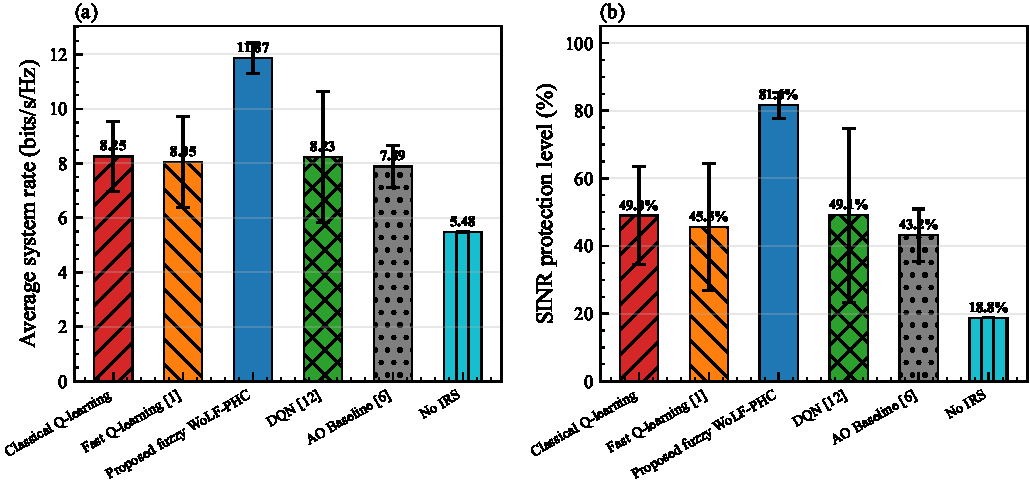
\includegraphics[width=\columnwidth]{ieee_fig9_evaluation.pdf}
\caption{Evaluation comparison: (a)~system rate and (b)~SINR protection (mean $\pm$ std, 5 seeds). Fuzzy WoLF-PHC (blue) achieves the highest performance with the smallest variance across both metrics.}
\label{fig:eval_bar}
\end{figure}

\subsection{Effect of Maximum Transmit Power}

Fig.~\ref{fig:pmax} shows rate/protection versus $P_{\max}\in\{25,32,40\}\,\text{dBm}$. WoLF-PHC rises from $1.72$ to $11.87\,\text{bits/s/Hz}$ and from $0\%$ to $81.6\%$, showing stronger scaling with available power than deterministic AO.

\begin{figure}[t]
\centering
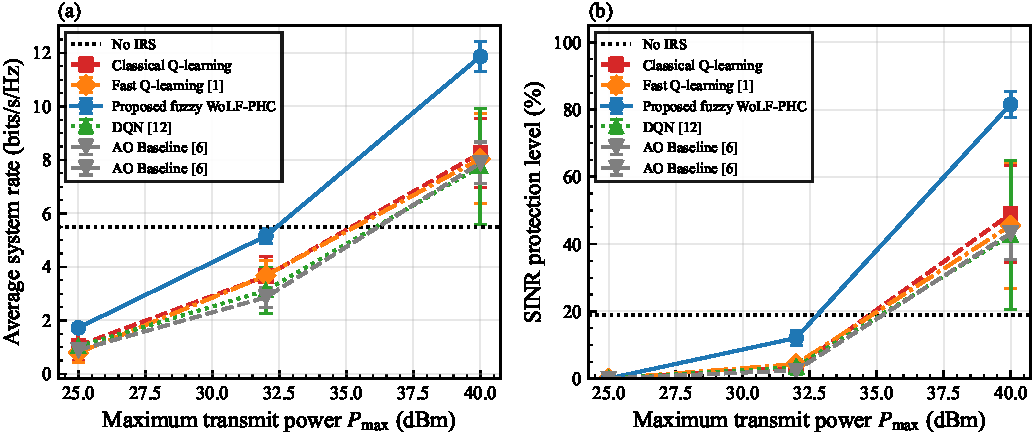
\includegraphics[width=\columnwidth]{ieee_fig5_vs_pmax.pdf}
\caption{(a)~System rate and (b)~SINR protection vs.\ maximum transmit power $P_{\max}$. WoLF-PHC scales most effectively with power, opening a gap over deterministic and tabular RL baselines at $40\,\text{dBm}$.}
\label{fig:pmax}
\end{figure}

\subsection{Effect of RIS Array Size}

Fig.~\ref{fig:nris} studies $N_\mathrm{RIS}\in\{16,64,144,256\}$. WoLF-PHC improves from $11.47$ to $11.87\,\text{bits/s/Hz}$ and from $79.2\%$ to $81.6\%$, confirming consistent gains with larger IRS size, with expected saturation at high element counts.

\begin{figure}[t]
\centering
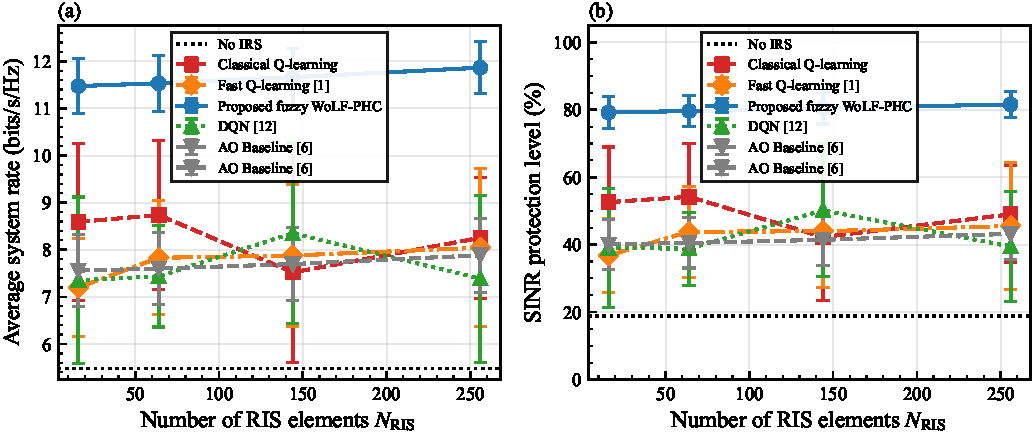
\includegraphics[width=\columnwidth]{ieee_fig6_vs_nris.pdf}
\caption{(a)~System rate and (b)~SINR protection vs.\ IRS array size $N_\mathrm{RIS}$. Performance grows with array size but saturates near $N_\mathrm{RIS}=256$; WoLF-PHC retains a consistent advantage at all scales.}
\label{fig:nris}
\end{figure}

\subsection{Effect of SINR Threshold}

Fig.~\ref{fig:sinr} evaluates $\gamma_{\min}\in\{3,5,10,15,20\}\,\text{dB}$. WoLF-PHC maintains the best trade-off across thresholds: $91.8\%$ protection at $3$~dB, $81.6\%$ at $5$~dB, and $31.4\%$ at $10$~dB. All methods collapse at $20$~dB, indicating a hard operating limit under the considered jammer.

\begin{figure}[t]
\centering
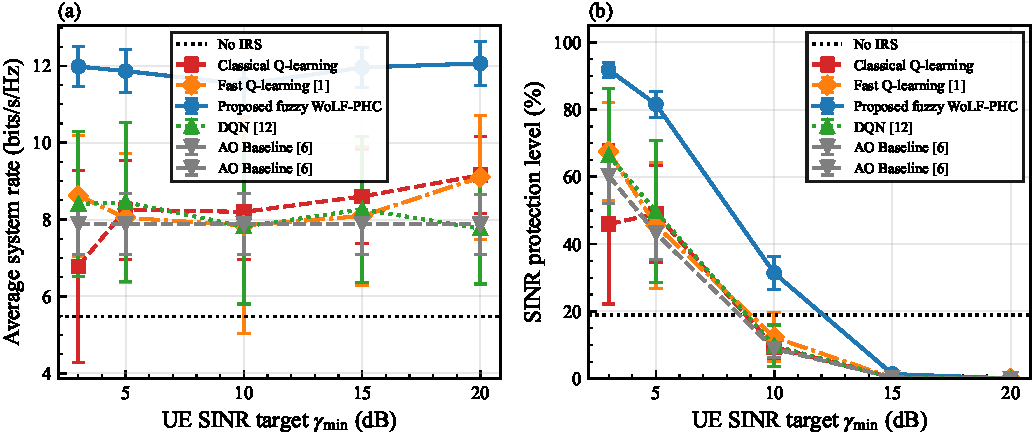
\includegraphics[width=\columnwidth]{ieee_fig7_vs_sinr.pdf}
\caption{(a)~System rate and (b)~SINR protection vs.\ UE SINR target $\gamma_{\min}$. WoLF-PHC shows the most graceful degradation with increasing SINR threshold, retaining $31.4\%$ protection at $10\,\text{dB}$.}
\label{fig:sinr}
\end{figure}

\subsection{Robustness to Jammer Power}

Fig.~\ref{fig:pjammer} shows a regime transition versus $P_J\in\{5,10,15,20\}\,\text{dBm}$. AO is competitive at low jammer power, but WoLF-PHC dominates for $P_J\geq15$~dBm and reaches $70.2\%$ protection at $20$~dBm, highlighting the value of mixed-strategy unpredictability.

\begin{figure}[t]
\centering
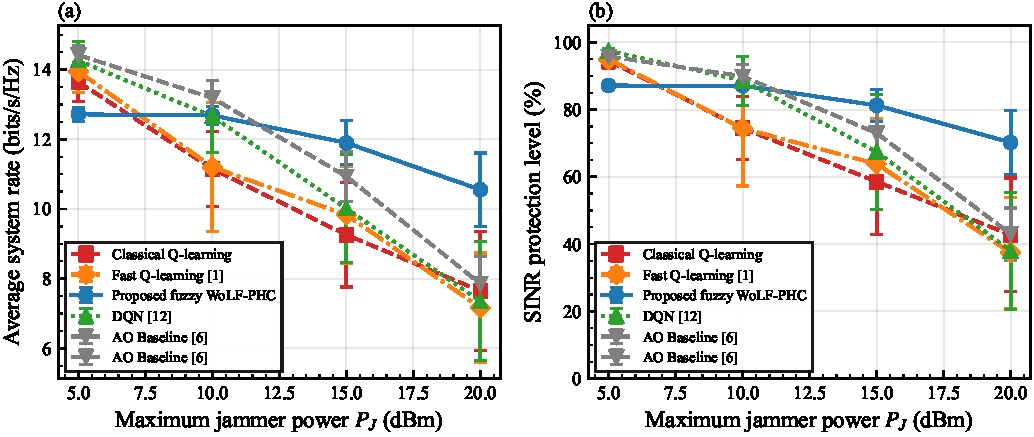
\includegraphics[width=\columnwidth]{ieee_fig12_vs_pjammer.pdf}
\caption{(a)~System rate and (b)~SINR protection vs.\ maximum jammer power $P_J$. A clear regime transition occurs near $10$--$15\,\text{dBm}$: WoLF-PHC's advantage grows with jammer power, while deterministic AO degrades sharply.}
\label{fig:pjammer}
\end{figure}

\subsection{Discussion}

Results confirm three points: WoLF-PHC gives the best and most stable rate/protection trade-off; robustness gains are largest in medium/high-jammer regimes; and larger IRS sizes provide consistent, though saturating, improvements.

% ══════════════════════════════════════════════════════════════════════
\section{Conclusion}
\label{sec:conclusion}
% ══════════════════════════════════════════════════════════════════════

This paper presented a three-block RL+AO framework for IRS-assisted anti-jamming in wideband THz systems, jointly optimizing power allocation, SPDP-RIS phases, and hybrid beamforming against an adaptive jammer. The proposed fuzzy WoLF-PHC controller achieved $11.87\,\text{bits/s/Hz}$ and $81.6\%$ SINR protection, improving over the best baseline by $44\%$ in rate and $66\%$ in protection with the lowest seed variance.

Parameter sweeps over $P_{\max}$, $N_\mathrm{RIS}$, $\gamma_{\min}$, and $P_J$ confirm robust gains and a clear regime transition: deterministic AO is competitive at low jammer power, while WoLF-PHC is superior in medium/high-jammer regimes. Future work will address imperfect CSI, multi-cell coupling, and near-field THz IRS modeling.

% ══════════════════════════════════════════════════════════════════════
% REFERENCES
% ══════════════════════════════════════════════════════════════════════

\begin{thebibliography}{99}

\bibitem{yang2021irs}
H.~Yang, Z.~Xiong, J.~Zhao, D.~Niyato, Q.~Wu, H.~V.~Poor, and M.~Tornatore,
``Intelligent reflecting surface assisted anti-jamming communications: A fast reinforcement learning approach,''
\emph{IEEE Trans.\ Wireless Commun.}, vol.~20, no.~3, pp.~1963--1976, Mar.\ 2021.

\bibitem{liang2019secure}
Y.~Liang, H.~V.~Poor, and S.~Shamai,
``Information theoretic security,''
\emph{Found.\ Trends Commun.\ Inf.\ Theory}, vol.~5, no.~4--5, pp.~355--580, 2009.

\bibitem{hanawal2016joint}
M.~K.~Hanawal, M.~J.~Abdel-Rahman, and M.~Krunz,
``Joint adaptation of frequency hopping and transmission rate for anti-jamming wireless systems,''
\emph{IEEE Trans.\ Mobile Comput.}, vol.~15, no.~9, pp.~2247--2259, Sep.\ 2016.

\bibitem{xu2018jamming}
Y.~Xu, G.~Ren, J.~Chen, Y.~Luo, and L.~Jia,
``Anti-jamming transmission in cognitive radio networks with unknown channel statistics,''
\emph{IEEE Trans.\ Wireless Commun.}, vol.~17, no.~2, pp.~765--779, Feb.\ 2018.

\bibitem{li2015relay}
X.~Guan, Q.~Wu, and R.~Zhang,
``Intelligent reflecting surface assisted secrecy communications: Is artificial noise helpful or not?''
\emph{IEEE Wireless Commun.\ Lett.}, vol.~9, no.~6, pp.~778--782, Jun.\ 2020.

\bibitem{wu2019intelligent}
Q.~Wu and R.~Zhang,
``Intelligent reflecting surface enhanced wireless network via joint active and passive beamforming,''
\emph{IEEE Trans.\ Wireless Commun.}, vol.~18, no.~11, pp.~5394--5409, Nov.\ 2019.

\bibitem{wu2021irs_survey}
Q.~Wu, S.~Zhang, B.~Zheng, C.~You, and R.~Zhang,
``Intelligent reflecting surface-aided wireless communications: A tutorial,''
\emph{IEEE Trans.\ Commun.}, vol.~69, no.~5, pp.~3313--3351, May 2021.

\bibitem{renzo2020smart}
M.~Di~Renzo \emph{et al.},
``Smart radio environments empowered by reconfigurable intelligent surfaces: How it works, state of research, and the road ahead,''
\emph{IEEE J.\ Sel.\ Areas Commun.}, vol.~38, no.~11, pp.~2450--2525, Nov.\ 2020.

\bibitem{su2023wideband}
X.~Su, G.~Wang, L.~You, and X.~Gao,
``Wideband precoding for RIS-aided THz communications,''
\emph{IEEE Trans.\ Commun.}, vol.~71, no.~10, pp.~5862--5876, Oct.\ 2023.

\bibitem{yan2023beamforming}
W.~Yan, W.~Yuan, X.~Kuai, and Z.~Wei,
``Beamforming analysis and design for wideband THz reconfigurable intelligent surface communications,''
\emph{IEEE J.\ Select.\ Areas Commun.}, vol.~41, no.~8, pp.~2306--2320, Aug.\ 2023.

\bibitem{watkins1992q}
C.~J.~C.~H.~Watkins and P.~Dayan,
``Q-learning,''
\emph{Machine Learning}, vol.~8, no.~3--4, pp.~279--292, 1992.

\bibitem{mnih2015human}
V.~Mnih \emph{et al.},
``Human-level control through deep reinforcement learning,''
\emph{Nature}, vol.~518, no.~7540, pp.~529--533, Feb.\ 2015.

\bibitem{bowling2002wolf}
M.~Bowling and M.~Veloso,
``Multiagent learning using a variable learning rate,''
\emph{Artif.\ Intell.}, vol.~136, no.~2, pp.~215--250, 2002.

\end{thebibliography}

\balance

\end{document}
